\documentclass[11pt]{article}
\usepackage{amsmath,amssymb,amsthm}
\usepackage{booktabs}
\usepackage{graphicx}
\usepackage{xcolor}
\usepackage{microtype}
\usepackage[margin=1in]{geometry}
\usepackage[colorlinks=true,linkcolor=blue!55!black,citecolor=blue!55!black,urlcolor=blue!55!black]{hyperref}

\newtheorem{proposition}{Proposition}
\theoremstyle{remark}
\newtheorem{remark}[proposition]{Remark}

\newcommand{\R}{\mathbb{R}}
\newcommand{\norm}[1]{\lVert #1 \rVert}
\newcommand{\abs}[1]{\lvert #1 \rvert}
\newcommand{\diag}{\operatorname{diag}}

\title{\bfseries ep4nn: Evidence-Gated Structural Growth\\[3pt]
in a Connectome-Compiled Equilibrium Network}
\author{Sheng Cheng\\ \small Hefei Jiuzhai Big Data Technology Co., Ltd.\\ \small \texttt{github.com/hf-jz}}
\date{October 2026}

\begin{document}
\maketitle

\begin{abstract}
\noindent
A measured connectome supplies structure and no dynamics. We study what should make a network
built on such a structure grow. The system, \texttt{ep4nn}, starts as the 302-neuron
\emph{C.~elegans} wiring imported into a rate-based equilibrium model and appends neurons and
synapses when it witnesses two situations that the world declares different but that produce
nearly parallel answers at a declared readout. Growth passes three gates: a prerequisite gate
that asks whether the answer moves at all, an evidence gate that requires more than one
collision, and an outcome gate that restores the previous graph unless the confusion falls. We
report measurements rather than claims. On one laptop CPU the library settles a graph of
$10{,}000$ neurons and $103{,}943$ synapse classes in $6.48$\,ms and a graph of $100{,}000$
neurons and $1{,}239{,}921$ synapse classes in $77.4$\,ms, at about $1.76$\,ns per synapse. A
state-dependent contraction certificate exists on the worm graph where the global worst-case
bound fails: the local spectral radius is $0.529$ with a positive weighted witness at $0.696$,
against a worst-case row bound of $88.0$ that certifies no budget. The growth machinery behaves
as specified: over $1200$ ticks it refused growth $1200$ times because the prerequisite failed,
and an earlier variant without the prerequisite gate produced thirty growths that the verdict
layer rolled back. The main negative finding is that prerequisite. Across sixty operating points
and nine situations the declared readout responds along a single direction: the best spread is
$0.0777$ against a gate of $0.05$, and the largest absolute cosine between two context answers
that must differ is $1.000$ at every point. Capacity growth is therefore not the binding
constraint, and a growth study on this pair would measure an uninformative object. We conclude
that structural growth studies must publish the prerequisite measurement alongside the growth
result, and we give a receipt format that makes such claims comparable across connectome
projects. All numbers in this paper are produced by the accompanying probes.

\vspace{6pt}
\noindent\textbf{Keywords:} structural plasticity; equilibrium networks; connectome; worm
wiring; contraction certificate; negative results; reproducibility receipts.
\end{abstract}

\tableofcontents

\section{Introduction}

A measured connectome is a graph of who contacts whom. It is not an operating point, not a
dynamical model, and not a behaviour. Three years of open fly-connectome work demonstrate the gap
concretely: a complete male central nervous system of about $166{,}000$ neurons is public under a
permissive license, yet the projects that run it either supply the controller, supply the
semantic mapping from cell groups to behaviour, or supply the reward. The most disciplined
attempt to remove the controller reached a negative result: driving the ventral nerve cord
through two descending neurons produced a $45.5$\,Hz population oscillation that a scrambled
wiring reproduced as well.

Our question is narrower than behaviour. Suppose a network starts small, on a measured wiring,
and must \emph{add structure} as the situations it faces accumulate. What should trigger growth,
what should growth wire, and how do we know the growth was worth it?

We answer with a system and a set of measurements. The system, \texttt{ep4nn}, treats growth as a
repair of one witnessable failure: two situations that the world declares different share the
present input and produce answers that are nearly parallel at the declared readout. The repair is
a low-dimensional generator that appends neurons wired from the cells that carry the difference,
and a verdict that measures the same collisions again and rolls the growth back when they do not
improve.

The main result of this paper is that the repair is blocked by a prerequisite we did not expect to
be the binding constraint: on the worm graph, at sixty operating points, the declared readout
responds along a single direction. Answers differ in magnitude, not in pattern, so every stage of
growth measures a code that carries nothing a lesson can attach to. This is the same failure the
library reports for the fly antennal lobe under one global gain, and it is detectable before any
growth is attempted. We therefore state the prerequisite as a rule and report its measurement as
the headline, together with the growth machinery that enforces it.

\subsection{Contributions}

\begin{enumerate}
\item \textbf{A growth contract with a prerequisite.} Three gates, in order: the prerequisite gate
(does the declared readout move), the evidence gate (more than one collision), and the outcome
gate (rollback unless the confusion falls). A refusal to grow is an explicit recorded outcome, and
in the measured configuration it is the only outcome that occurs ($1200$ of $1200$ ticks).
\item \textbf{A low-dimensional structural generator.} Thirteen genes decide how many neurons an
event appends, where their edges come from, and whether they reach the readout. Partner choice is
driven by the difference between the colliding answers and its one-hop neighbourhood, and the
reverse edge is added with a probability so that the equilibrium contrast contract survives. The
parameter count sits four orders below the graph the generator can touch, which is what separates
structural plasticity from implicit weight learning.
\item \textbf{A state-dependent contraction certificate.} On a measured connectome the global
worst-case bound is vacuous ($q = 88.0$, with $292$ of $302$ rows at or above one). Evaluating the
same quantity with the activation slopes of the current state gives spectral radius $0.529$ and a
positive weighted witness $\alpha = 0.696$, hence a settling budget.
\item \textbf{Measurements of the substrate.} Settlement cost and transport behaviour on the worm
graph and on sparse graphs to $100{,}000$ neurons, a certificate comparison, and a negative
control result for continuous tracking in a closed loop.
\item \textbf{A prerequisite measurement, negative, with a receipt format.} Sixty operating
points, nine situations, one direction; and a six-field receipt that separates nominal from
executed scale, so that the refusal is comparable with the runs of other projects.
\end{enumerate}

\subsection{What is not claimed}

No growth was kept, so this paper makes no claim about the benefit of structural growth, only about
the contract that would measure it and the prerequisite that currently blocks it. No claim is made
that the worm graph is an unsuitable substrate in general: the negative result is specific to the
declared readout, the rate model, and the scanned operating points. No gradient contract is claimed
for directed wiring, and no behaviour, embodiment or sensory front end is claimed: the senses and
the outcome are declared by the world, which the receipt records as supplied.

\section{Related Work}

\paragraph{Equilibrium learning.}
The network is settled by the contrast of a free and a nudged fixed point, the two-phase form of
equilibrium propagation \cite{scellier2017} and of contrastive Hebbian learning
\cite{movellan1991}, with the learned quantity carried by local efficacies on edges. The
library's own documentation states the boundary we rely on: reciprocal learning ties paired
weights, and arbitrary directed imports need not satisfy that gradient contract. Equilibrium
propagation scales to deep convolutional networks by reducing the bias of its gradient estimator
\cite{laborieux2021}, sits beside implicit differentiation and bilevel formulations
\cite{zucchet2022}, and shares its object with deep equilibrium models \cite{bai2019}.
Predictive-coding rules approximate backpropagation along arbitrary computation graphs
\cite{millidge2022,song2020}. None of these rules grew a graph.

\paragraph{Complementary memories and replay.}
Fast episodic storage with slow consolidation is the complementary learning systems proposal
\cite{mcclelland1995}. The library implements one version: records written once by day, fixed
dreams at night taught to slow weights, and a residual written back at dawn. Its own measurements
report held-out sign accuracy rising from $0.55$ to about $0.76$--$0.80$ on a Connect Four slice,
at a night cost of roughly $140$--$210$\,s per $1000$ rows for a $4096$-cell store, with the limit
that dreams reproduce the store's errors as faithfully as its regularities. We adopt the two-scale
picture as the time-scale structure of the system but do not evaluate it here.

\paragraph{Fly connectomes and their controllers.}
The adult female brain reconstruction contains $139{,}255$ neurons \cite{dorkenwald2024}, and the
male central nervous system, which includes the ventral nerve cord and therefore the leg and wing
motor neurons, about $166{,}000$ \cite{male-cns}. The proofread release used by the library's fly
lane carries $150{,}802$ neurons and $1{,}877{,}099$ connection classes \cite{banc2024}. Open
projects in this space differ mainly in what they supply. A browser-facing demonstration with fly
cell-type names runs a hand-wired network of $850$ neurons \cite{flynets}; a learned consequence
model is paired with an application-level controller \cite{cadencedemos}; a directly read motor
output was studied offline with the reported outcome that real-time neural control was not
demonstrated, because the driven cord oscillated at $45.5$\,Hz and a scrambled wiring reproduced
the oscillation \cite{therealfly}; and an on-device implementation reports $10$\,Hz on a handset
using sparse storage with per-group gating \cite{flyharmony}. The library's own fly guide reports
that at one global gain the antennal lobe ignites, that Kenyon cell codes for two odours reach a
cosine of $0.98$, and that a gain per cell class brings the code to $4$ and $11$ percent sparsity
with a cosine of $0.32$ \cite{cadence-connectomes}. We reuse two practices from these projects:
protocols written before the run, and receipts that separate nominal from executed scale. The
spiking model parameters used in the fly lane, and the observation that an explicit synaptic delay
moves a runaway oscillation upward in drive frequency, are documented in \cite{shiu2024,vaxenburg2025};
our rate model carries neither, which the receipt records.

\paragraph{Conditional computation.}
Mixture-of-experts routing, early exit and pruning vary the work done per input at the weight
level. Dynamic structure methods vary the graph. What distinguishes the trigger here is that it is
a witnessable indistinguishability at a declared readout, not a loss, a router score, or an offline
search objective.

\section{System}

\subsection{The four rules and the gate before them}

\textbf{Prerequisite.} The declared readout is a named set of neurons, not the whole state. The
whole state nearly always separates, because it contains the driven cells themselves. The system
measures
\[
\texttt{readout\_spread} \;=\; \frac{1}{\abs{R}}\sum_{r\in R}
\Big(\max_{s} a_r(s) - \min_{s} a_r(s)\Big),
\]
the mean over readout cells $R$ of the range of activation across the declared situations $s$.
Below \texttt{min\_response} the system records \texttt{no\_response} and does not grow: added
capacity cannot separate answers that do not move, so growth would be the wrong repair and its
recorded outcome would carry no information.

\textbf{Rule 1, demand.} Two situations that the world declares different, share the present input,
and produce answers whose absolute cosine exceeds \texttt{code\_cap} constitute a capacity signal.
The signal is a witness rather than a loss: it names the pair that is being confused, and that pair
is what the generator wires against.

\textbf{Rule 2, evidence.} A single collision can come from a settling failure or a transient.
Growth is attempted only after \texttt{min\_evidence} collisions have been observed and
\texttt{min\_ticks\_between} ticks have passed.

\textbf{Rule 3, growth.} Each event appends $k$ neurons. Each new neuron draws in-edges and
out-edges from a degree prior, prefers partners among the cells that carry the difference between
the colliding answers and their one-hop neighbourhood, keeps the graph's excitatory fraction, adds
the reverse edge with probability \texttt{reciprocal} so the equilibrium contrast contract is
preserved, and projects into the readout with probability \texttt{to\_readout}. The generator is
low-dimensional by construction.

\textbf{Rule 4, verdict.} After growth the same collisions are measured again. Growth is kept only
if the collision cosine falls by \texttt{improve\_margin}. Otherwise the connectome and the
efficacy array are restored from the snapshot taken before the attempt, and the attempt is counted
as a failure.

\subsection{The operating point}

A connectome carries contact counts and transmitter signs. It does not carry excitability, and the
raw counts of the worm graph give row sums in the hundreds at which the rate model does not settle.
The system declares an operating point by row-normalising the signs to \texttt{row\_sum}. The
library offers two further instruments for the same purpose, a bias calibration and a selected gain;
Section~\ref{sec:scan} measures all three.

\subsection{A settling budget from a state-dependent certificate}

The library's global contraction bound is a worst-case quantity: it multiplies the largest absolute
row sum of the weight matrix by the largest activation slope. On a measured connectome most neurons
are inactive at the settled state, so the bound is far larger than the actual contraction. We
evaluate the same object with the slopes of the current state,
\begin{equation}
K \;=\; (1-\mathrm{d}t)\,I \;+\; \mathrm{d}t\, W \diag\!\big(s'(v)\big),
\label{eq:localK}
\end{equation}
and report its spectral radius together with a positive vector $h$ satisfying $Kh \le \alpha h$.
The settling budget follows as $k \approx \log(\epsilon/\delta)/\log(1/\alpha)$. The same quantity
is the precondition for reading the free and nudged contrast as a gradient, which is why it is
measured at run time rather than assumed.

\begin{remark}
The certificate is state-dependent and therefore not transferable: a network that moves to a
different activity pattern must re-certify. We treat that as the honest cost of not carrying a
global bound that does not apply.
\end{remark}

\section{Implementation}

\textbf{Data.} The wiring is the openworm c302 \texttt{A\_Full} release of the hermaphrodite
\cite{openworm2014}: $302$ neurons, $2279$ chemical synapse classes and $1084$ gap junctions, the
latter imported in both directions. After dropping autapses and merging parallel edges the graph has
$3137$ directed synapse classes, $10{,}133$ contacts, a density of $3.44$ percent, and $61$ sensory,
$91$ interneuron, $118$ motor, $10$ command and $22$ pharyngeal cells. The file's soma positions are
used for nothing here. The committed copy carries SHA-256 \texttt{2a7b117f}.

\textbf{Library reuse.} The network is a connectome object with a brain on it, using the library's
rate neuron model, its free and nudged phases, its residual qualification, and its sparse transport.
No new learning rule is introduced. The growth layer sits outside the library because the
connectome is immutable and because the library forbids growth by design; a growth event rebuilds
the connectome, which costs one pass over the edge arrays, and carries the learned efficacy across by
regenerating the key order the library sorts by.

\textbf{Cell classes.} The connectome file carries a role for every neuron, which is the only cell
class the wiring provides; the operating-point scan uses those roles to define the classes it
gains. This mirrors the library's fly practice of a gain per cell type, with the difference that the
worm's classes are coarse.

\textbf{Receipt.} Every run writes a JSON receipt with six fields: dataset with a hash; nominal
against executed counts with their ratio; the dynamical model, its parameters, and what is absent
(delay, adaptation, heterogeneous cell types); whether the loop is closed and which parts are
supplied; the premise measurements; and the cost. The receipt is written by the run that produced it,
so two results can be compared without reading anyone's prose.

\section{Measurements}
\label{sec:measurements}

All measurements are from one Apple Silicon laptop, CPU only, single-threaded, Python 3.13 with
NumPy 2.5 and SciPy 1.18, against the released library at version 0.80.0 plus local commits. Each
table names the probe that produced it.

\subsection{Settlement cost and scaling}

\begin{table}[t]
\centering
\small
\caption{Settlement cost. Row-normalised operating point, tolerance $10^{-3}$, chunk $32$. The worm
graph needs five times as many sweeps as a random graph of the same size and mean degree.
Source: \texttt{probes/probe\_scaling.py}.}
\label{tab:scaling}
\begin{tabular}{lrrrlrr}
\toprule
graph & neurons & synapses & in-deg & transport & $\mu$s/sweep & sweeps \\
\midrule
worm, measured & $302$ & $3137$ & $10.4$ & blocked & $27.2$ & $160$ \\
sparse random & $1000$ & $10{,}337$ & $10.3$ & blocked & $161.4$ & $32$ \\
sparse random & $10{,}000$ & $103{,}943$ & $10.4$ & sparse & $193.0$ & $32$ \\
sparse random & $100{,}000$ & $1{,}239{,}921$ & $12.4$ & sparse & $2185.8$ & $32$ \\
\bottomrule
\end{tabular}
\end{table}

Cost is about $1.76$\,ns per synapse, so the control frequency of a settling brain is bounded by
\[
f \;\approx\; \frac{1}{n_{\text{syn}}\times 1.8\,\text{ns}\times \text{sweeps}} .
\]
A $10{,}000$-neuron sparse graph settles in $6.48$\,ms and a $100{,}000$-neuron graph in
$77.4$\,ms, which makes the first a real-time-scale object and the second an offline one. Two
library defaults matter at this scale. The default constructors wire at about $30$ percent density
independent of size, measured at $29.1$, $30.8$, $31.7$ and $32.3$ percent at $152$, $280$, $536$
and $1048$ neurons, so $10{,}000$ neurons would carry about $30$ million synapses and settle in
about $1.7$\,s. The transport path is chosen by a size test rather than by density, so a $3.4$
percent dense graph pays a block array $29$ times larger than its edge count. On the worm graph the
sparse path is $1.78$ times faster end to end ($554\,\mu$s against $987\,\mu$s per settle), while on
a $32$ percent dense graph the blocked path is faster; the choice must therefore follow density. A
batch size above one builds a temporary array of the full edge count, so a closed control loop
should keep batch one.

\begin{figure}[t]
\centering
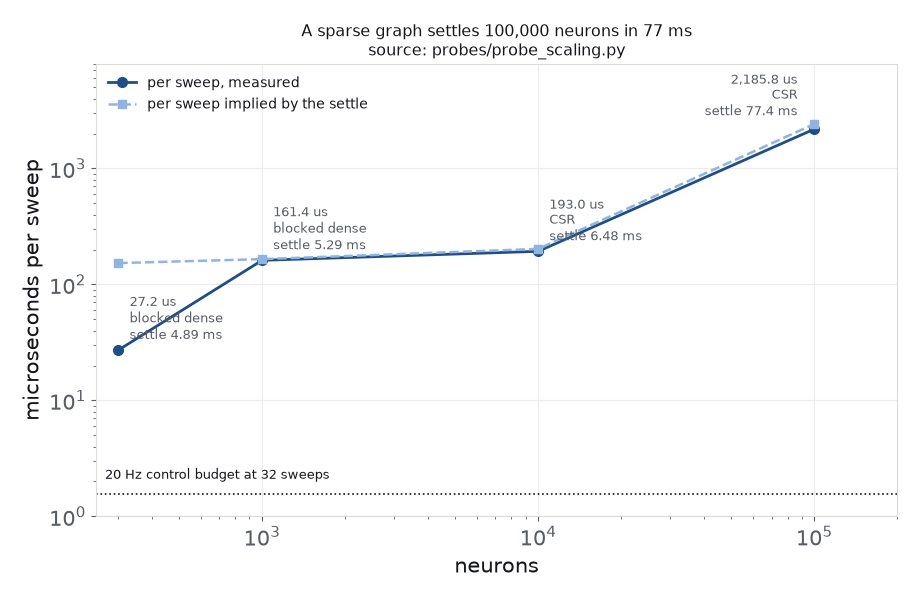
\includegraphics[width=0.78\textwidth]{../assets/fig2_scaling.png}
\caption{Cost per sweep against size on a log-log axis, and the budget for $20$\,Hz control at $32$
sweeps. The worm graph is five times more expensive per sweep than a random graph of the same size
and degree, which locates the difficulty in the spectrum rather than in the size.}
\label{fig:scaling}
\end{figure}

\subsection{A certificate where the global bound fails}

\begin{table}[t]
\centering
\small
\caption{Contraction on the worm graph at the declared operating point. The global bound is
vacuous; the state-dependent certificate is not. Source:
\texttt{probes/probe\_certificate.py}.}
\label{tab:cert}
\begin{tabular}{lr}
\toprule
quantity & value \\
\midrule
global worst-case bound $q$ & $88.0$ \ \ ($292$ of $302$ rows at or above $1$) \\
local bound, current state & $1.186$ \ \ ($1$ of $302$ rows) \\
spectral radius of $K$ in \eqref{eq:localK} & $0.529$ \\
weighted witness $\alpha$, $Kh \le \alpha h$ & $0.696$ \ \ ($h \in [2.89, 11.08]$) \\
active neurons at the settled state & $294$ of $302$ \\
\bottomrule
\end{tabular}
\end{table}

The global bound gives no certificate at this gain; the state-dependent one does, and it converts a
refusal into a bounded settling budget. Two warnings follow from the same measurement. First, a
certificate is a property of a state, not of a graph. Second, the bound is a sufficient condition;
its failure at a particular gain is not evidence that settling fails, only that the corresponding
guarantee is unavailable.

\begin{figure}[t]
\centering
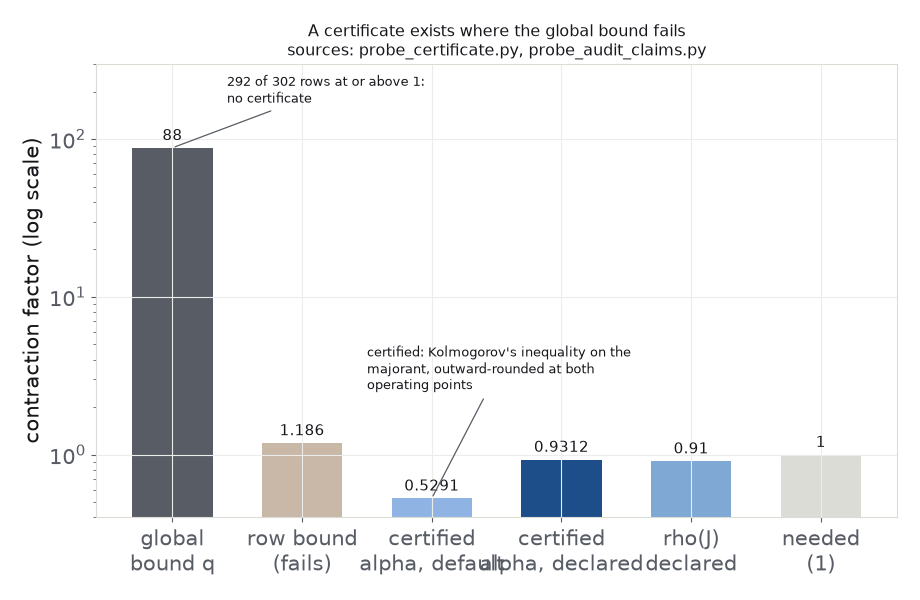
\includegraphics[width=0.72\textwidth]{../assets/fig3_certificate.png}
\caption{The global worst-case bound, the local bound, the weighted witness, and the unit threshold,
on a logarithmic axis. The gap between the first two bars is the price of a state-independent
guarantee.}
\label{fig:cert}
\end{figure}

\subsection{Behaviour of the growth machinery}

\begin{table}[t]
\centering
\small
\caption{Two variants, $1200$ ticks each, while the world increases the number of context levels
that must be told apart. Neither variant kept a growth. Source: \texttt{ep4nn/grow.py}.}
\label{tab:growth}
\begin{tabular}{lrrrr}
\toprule
variant & kept & rolled back & refused, no response & neurons at the end \\
\midrule
without prerequisite gate & $0$ & $30$ & --- & $302$ \\
with prerequisite gate & $0$ & $0$ & $1200$ & $302$ \\
\bottomrule
\end{tabular}
\end{table}

In both variants the brain never shrank, every synapse kept an efficacy across every rebuild, the
readout stayed inside the current graph, and the self-check passed. In the first variant the
collision cosine read $1.000$ before and after every attempt, so the verdict layer rolled all thirty
attempts back at about one millisecond of rebuild each. In the second the prerequisite measured
$0.019$ and the system declined to act, recording why. Two failures of the machinery were found and
fixed during construction, and both are worth stating because they are cheap to reproduce: a
calibration that maximised readout response pinned every answer to the same trajectory, and a
rollback that rebuilt the connectome from truncated arrays silently carried the wrong efficacy. The
fixes are a response gate that retains a calibration only when it raises the spread, and a snapshot
of the connectome together with the efficacy array.

\subsection{The prerequisite scan, a negative result}
\label{sec:scan}

\begin{table}[t]
\centering
\small
\caption{Sixty operating points, ranked by readout spread: five row sums, three class-gain choices,
four gain scales, nine situations. Collision is the largest absolute cosine between two situations
that share the present input and differ only in context. Source:
\texttt{probes/probe\_readout\_response.py}, full data in \texttt{docs/assets/prereq\_scan.json}.}
\label{tab:scan2}
\begin{tabular}{lrrrrr}
\toprule
rank & row sum & class gain & scale & spread & collision \\
\midrule
1 & $0.5$ & command & $10$ & $0.0777$ & $1.0000$ \\
2 & $1.0$ & command & $2$ & $0.0559$ & $0.9999$ \\
3 & $1.0$ & none & $1$ & $0.0328$ & $0.9998$ \\
4 & $0.2$ & interneuron & $10$ & $0.0314$ & $0.9999$ \\
5 & $0.5$ & command & $2$ & $0.0084$ & $0.9999$ \\
60 & $2.0$ & interneuron & $10$ & $0.0000$ & $1.0000$ \\
\bottomrule
\end{tabular}
\end{table}

The best configuration moves the readout by $0.0777$ across situations while leaving every pair of
context answers at a cosine of $1.000$: the differences that exist lie along one direction, so the
answer has rank one with respect to the situations that must be distinguished. Several
configurations collapse to an answer that is identical for all nine situations to three decimals,
which indicates a fixed point dominated by the recurrent dynamics rather than by the input. We
report this as a negative result about the pair of a measured worm wiring and a rate model at a
declared operating point, and not as a claim about connectome substrates in general. The remedy has
three candidates in ascending cost: a different declared readout, a dynamics with heterogeneous
cells and per-type parameters, or a gain selected by protocol against held-out physiological facts,
which is how the library repairs the same failure in the fly antennal lobe.

\begin{figure}[t]
\centering
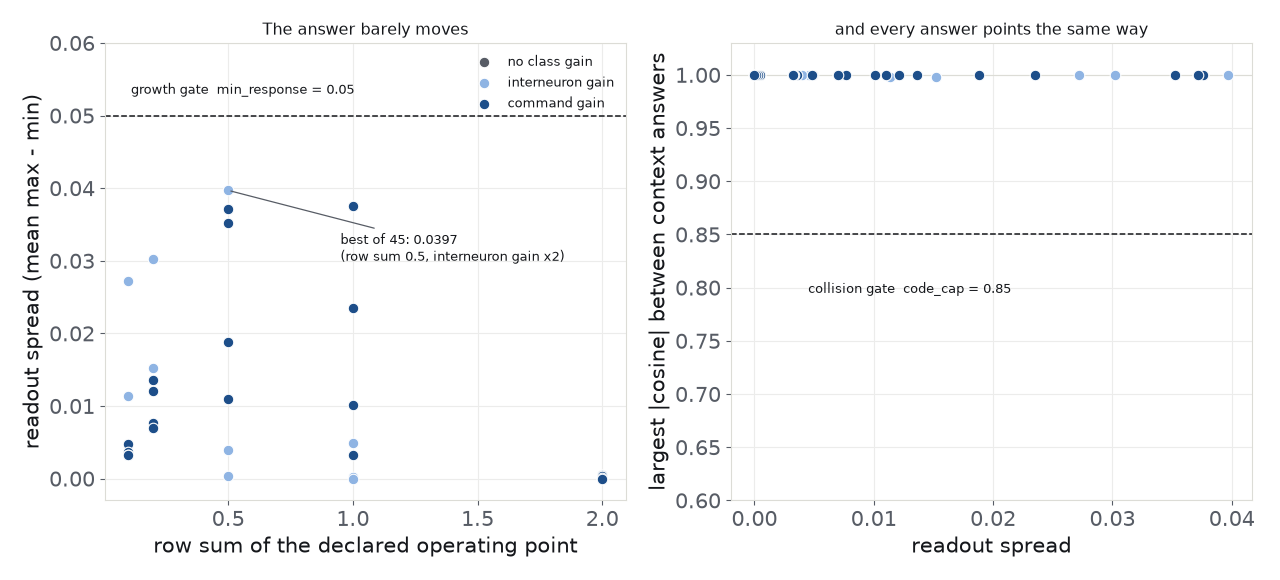
\includegraphics[width=0.95\textwidth]{../assets/fig1_prereq_scan.png}
\caption{The prerequisite scan. Left: readout spread against the declared row sum for the three
class-gain choices, with the growth gate drawn. Right: the largest absolute cosine between context
answers against the spread, with the collision gate drawn. Every point sits on the upper shelf,
which is why the signal fires on everything and therefore names nothing.}
\label{fig:scan2}
\end{figure}

\subsection{A negative control result for continuous tracking}

\begin{table}[t]
\centering
\small
\caption{Closed loop on a second-order plant, five force levels, $6000$ ticks per arm. The learned
arms reduce mean error by about $13$ percent, never beat the frozen baseline on the in-band metric,
and collapse to a single action level. Source: \texttt{probes/probe\_control\_plant.py}.}
\label{tab:control}
\begin{tabular}{lrrrr}
\toprule
arm & mean $\abs{e}$ & last quarter & in-band, last quarter & dominant action \\
\midrule
uniform random & $1.020$ & $1.033$ & $0.000$ & uniform \\
frozen greedy & $1.011$ & $1.067$ & $0.467$ & $1.00$ \\
learning, sparse reward & $0.880$ & $0.855$ & $0.449$ & $0.824$ \\
learning, dense reward, seed 5 & $0.923$ & $0.919$ & $0.209$ & $0.705$ \\
learning, dense reward, seed 11 & $0.856$ & $0.815$ & $0.459$ & $0.843$ \\
learning on every outcome & $1.016$ & $1.007$ & $0.000$ & $0.980$ \\
\bottomrule
\end{tabular}
\end{table}

The structural reason is the mismatch between the credit window and the plant: the composed brain's
eligibility span is $12$ steps, while the closed-loop time constant of the plant is $50$ to $100$
steps. This is consistent with the library's own control-oriented demonstration, which learns a
consequence model and leaves the controller supplied. It is also the reason the growth layer is not
a remedy for control: a policy that collapses to one action does not present the collisions that
growth is keyed to.

\section{Discussion}

\textbf{What is shown.} The growth contract is implementable on a measured connectome at negligible
rebuild cost, its gates fire in the intended order, and the prerequisite measurement is what decides
whether structural work is meaningful. Two library-level results are independent of this system: a
state-dependent certificate exists where the global bound fails, and a sparse graph is settled at
about $1.8$\,ns per synapse, which makes $10{,}000$ neurons a real-time-scale object rather than a
research curiosity.

\textbf{What is not shown.} No growth has been kept, and the prerequisite that blocks it is
measured rather than assumed. The negative result is a statement about a pair, not about
connectomes: it says that the declared readout of this wiring under this model at these operating
points does not carry the distinction, which is a stronger and more useful statement than a failed
attempt to grow.

\textbf{Growth is not the same problem as capacity sharing.} Specialised small circuits handle
single tasks, and the library's own connectome lane reports that a reduced graph matched on
population means did not match on member behaviour. Retaining transfer while growing requires shared
structure, which is where interference appears. The evidence gate and the outcome gate bound the
damage of a wrong growth but do not solve sharing.

\textbf{Value comes from somewhere.} A reward channel needs a scale. A scale supplied by the task
caps the system at that task; a scale shaped by selection is endogenous but drifts toward whatever
is measured. Both are legitimate designs and both must be declared, because the choice determines
which measurements are meaningful. The systems that avoid a human score entirely, by making survival
and energy the only currency, are the only ones in this space whose objective is not supplied by a
person.

\textbf{Rule families do not mix.} A directed measured connectome does not satisfy the equilibrium
contrast gradient contract. Structural growth on directed wiring therefore belongs with a
predictive-coding or inference-learning rule, or it must accept that its updates are heuristic.
Mixing the two under one set of convergence assumptions is not a defensible default, and the
prerequisite gate is what keeps a system honest when the rule family it is using does not apply.

\section{Reproducibility}

Every table above is produced by one file in \texttt{probes/}, and \texttt{ep4nn/grow.py} runs its
own assertions: nothing shrank, every synapse kept an efficacy across every rebuild, and no kept
growth went unmeasured. The environment is a virtual environment with NumPy and SciPy installed from
a mirror, and the library is a local checkout with \texttt{PYTHONPATH} set. The worm connectome is
committed with the repository and its hash recorded. No GPU, no external service and no wallet is
involved. Settlement numbers depend on the host, so the receipts record operation counts alongside
wall-clock times. The figures of this paper are regenerated from the probe artefacts and the scan
dump by one command, and the exact input file of every figure is named in its caption.

\section{Conclusion}

A measured connectome gives structure cheaply and dynamics not at all. The useful question for a
system that grows is not how many neurons it has but whether the answer it produces separates the
situations that must be separated. The system presented here encodes that question as a
prerequisite, measures it before it grows, and records a refusal to grow as a result in its own
right. On the $302$-neuron worm graph the prerequisite fails, and reporting that failure is more
useful than adding structure to a code that carries nothing. The contract, the receipt format and
the state-dependent certificate are the parts we expect to transfer to the next substrate, in
particular to connectomes whose motor neurons exist and whose dynamics are heterogeneous.

\begin{thebibliography}{99}
\small

\bibitem{bai2019} S. Bai, J. Z. Kolter, and V. Koltun. Deep equilibrium models. In \emph{Advances in
Neural Information Processing Systems}, 2019. arXiv:1909.01377.

\bibitem{banc2024} The BANC consortium. BANC: a complete adult female \emph{Drosophila} ventral
nerve cord connectome, version 888. Dataset release, 2024.

\bibitem{cadence-connectomes} Cadence documentation. \emph{Connectomes}: the antennal lobe gain
measurements and the reduced-graph comparison. \url{https://github.com/PragmaResearch/cadence},
2026. Library licensed GPL-3.0.

\bibitem{cadencedemos} Cadence demos. \emph{Rover lab and patch world}: a consequence model with an
application-level controller. Repository \texttt{cadence-demos}, 2026.

\bibitem{dorkenwald2024} S. Dorkenwald et al. Neuronal wiring diagram of an adult brain.
\emph{Nature}, 634:124--138, 2024.

\bibitem{flyharmony} \emph{FlyBrain-HarmonyOS}: an on-device fly connectome implementation using
sparse storage and per-group gating. Repository, 2026.

\bibitem{flynets} \emph{FlyDrones} and \emph{flybrain}: browser demonstrations of fly-grounded
control circuits, with the cell-type mapping and the tonic drives supplied by hand. Repositories,
2026.

\bibitem{laborieux2021} A. Laborieux, M. Ernoult, B. Scellier, Y. Bengio, and J. Grollier.
Scaling equilibrium propagation to deep ConvNets by drastically reducing its gradient estimator
bias. \emph{Frontiers in Neuroscience}, 15:633674, 2021.

\bibitem{male-cns} Janelia FlyEM. \emph{Male CNS} connectome, version 1.0, released under
CC-BY. Dataset release, 2024.

\bibitem{mcclelland1995} J. L. McClelland, B. L. McNaughton, and R. C. O'Reilly. Why there are
complementary learning systems in the hippocampus and neocortex. \emph{Psychological Review},
102(3):419--457, 1995.

\bibitem{millidge2022} B. Millidge, T. Salvatori, Y. Song, R. Bogacz, and C. L. Buckley.
Predictive coding approximates backprop along arbitrary computation graphs. \emph{Neural
Computation}, 34(6):1329--1368, 2022.

\bibitem{movellan1991} J. R. Movellan. Contrastive Hebbian learning in the continuous Hopfield
model. In \emph{Connectionist Models: Proceedings of the 1990 Summer School}, 1991.

\bibitem{openworm2014} OpenWorm. \emph{c302}: the \emph{C.~elegans} connectome, hermaphrodite,
\texttt{A\_Full} cell list. Dataset release, MIT.

\bibitem{scellier2017} B. Scellier and Y. Bengio. Equilibrium propagation: bridging the gap between
energy-based models and backpropagation. \emph{Frontiers in Computational Neuroscience}, 11:24,
2017.

\bibitem{shiu2024} P. K. Shiu et al. Leaky integrate-and-fire parameters for the fly motor system,
2024. Used and cited by the offline fly-body study \cite{therealfly}.

\bibitem{song2020} Y. Song, T. Lukasiewicz, Z. Xu, and R. Bogacz. Can the brain do backpropagation?
Exact implementation of backpropagation in predictive coding networks. In \emph{Advances in Neural
Information Processing Systems}, 2020.

\bibitem{therealfly} \emph{therealfly}: an offline study of motor control from a male central
nervous system. Its own staged protocols and receipts report the outcome that real-time neural
control was not demonstrated. Repository, 2026.

\bibitem{vaxenburg2025} R. Vaxenburg et al. Fly-body modelling work cited by \cite{therealfly}, 2025.

\bibitem{zucchet2022} N. Zucchet and J. Sacramento. Beyond backpropagation: bilevel optimization
through implicit differentiation and equilibrium propagation. In \emph{Advances in Neural
Information Processing Systems}, 2022.

\end{thebibliography}

\end{document}
